\chapter{Site-instellingen}
\section{Actions}

Acties zijn individuele taken die door het systeem uitgevoerd kunnen worden, zoals publicatie 
van een pagina ongedaan maken of uitsluiten van een gebruiker. Modules, zoals de
Trigger-module, \index{trigger-module} kunnen deze acties starten wanneer
bepaalde systeemgebeurtennissen plaatsvinden; bijvoorbeeld wanneer een nieuw bericht wordt toegevoegd of wanneer een gebruiker inlogt. Modules kunnen 
voorzien in extra acties.
\\
Er zijn twee soorten acties: eenvoudige en geavanceerde. Eenvoudige acties behoeven geen extra 
configuratie en worden hier automatisch opgesomd. Geavanceerde acties kunnen meer dan eenvoudige 
acties, bijvoorbeeld een e-mail versturen naar een gespecificeerd adres, of inhoud controleren 
op bepaalde woorden. Deze acties moeten eerst worden aangemaakt en geconfigureerd voordat ze 
gebruikt kunnen worden. Selecteer een actie uit het keuzelijstmenu en klik op de knop Aanmaken 
om een geavanceerde actie aan te maken.
\begin{figure}[!h]
    \centering
   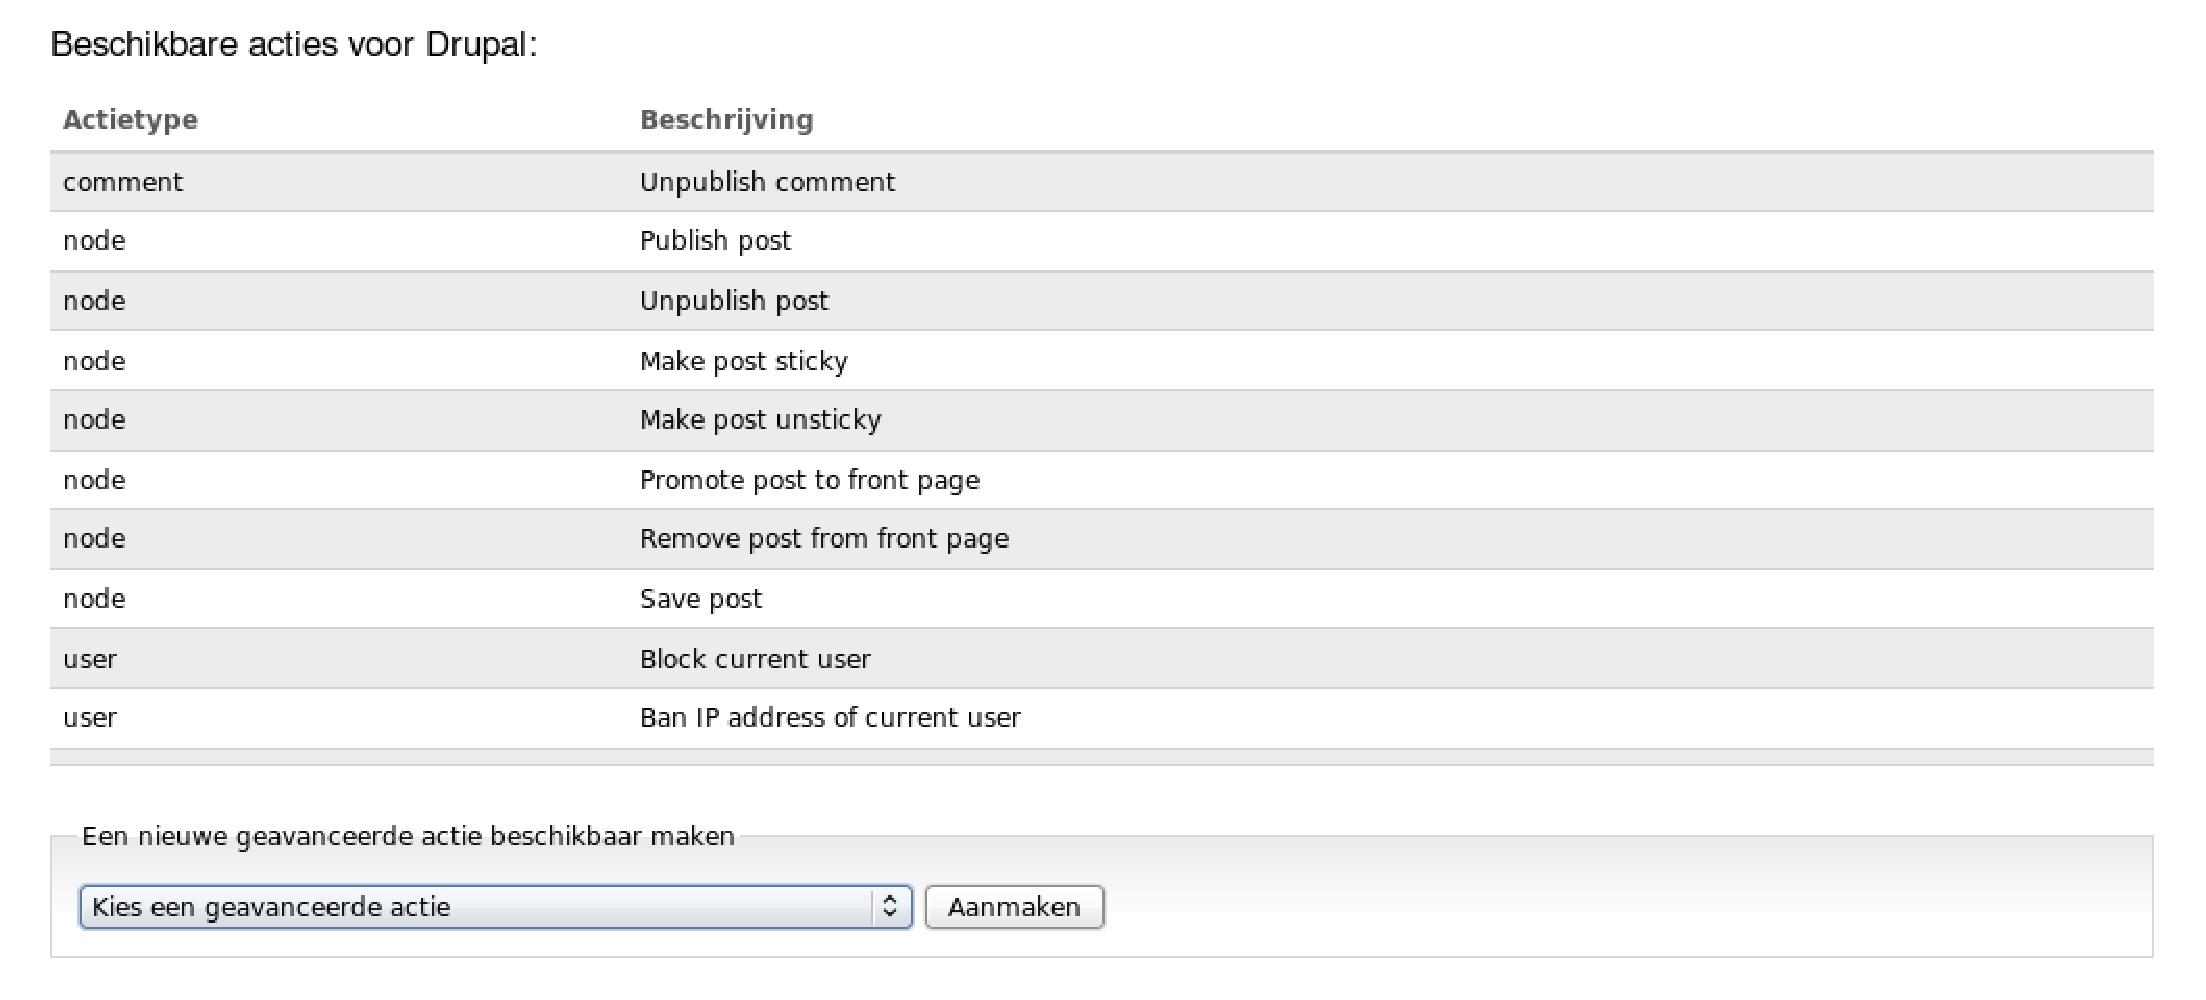
\includegraphics[scale=0.3,angle=0]{Actions}
   \caption{Actions.\label{white}}
 \end{figure}

\section{Administratiemenu} \index{administratiemenu}
De administratiemenu-module \index{administratiemenu-module} voorziet een
keuzelijstmenu dat met \'e\'en of twee klikken toegang biedt tot de meeste beheertaken en andere gemeenschappelijke bestemmingen (aan gebruikers met de gepaste 
toegangsrechten). Het administratiemenu toont eveneens het aantal anonieme en geverifieerde gebruikers 
en laat toe dat modules hun eigen menu-onderdelen toevoegen. Integratie van het menu hangt af van 
module tot module; bijvoorbeeld de uitbreidingsmodule Devel, maakt veel gebruik van de 
administratiemenu-module om snel toegang te geven tot de ontwikkelingshulpmiddelen.
\\
De Instellingenpagina van het admnistratiemenu laat toe om sommige onderdelen van het gedrag en het 
voorkomen van het menu te veranderen. Vermits het voorkomen van het menu afhankelijk is van het 
thema van uw site, vereisen aanzienlijke aanpassingen ook wijzigingen aan de thema- en CSS-bestanden 
van uw site. 
\\
De menu-onderdelen die worden weergegeven in het administratiemenu hangen af van de toegangsrechten 
van de gebruiker. Ten eerste, het administratiemenu wordt alleen getoond aan gebruikers in 
rollen met het Toegang administratiemenu (admin-menu module) toegangsrecht. Ten
tweede, een gebruiker moet deel uitmaken van een rol met de Toegang tot beheerpagina's (system module) 
toegangsrecht om de administratieve linken te bekijken. Ten laatste, alleen de huidig toegelaten 
linken worden getoond; b.v. indien een gebruiker geen lid is van een rol met het toegangsrecht 
Toegangsrechten beheren (user module) en Gebruikers beheren (user module), wordt het 
Gebruikerbeheer menu-onderdeel niet getoond.
\begin{figure}[!h]
    \centering
   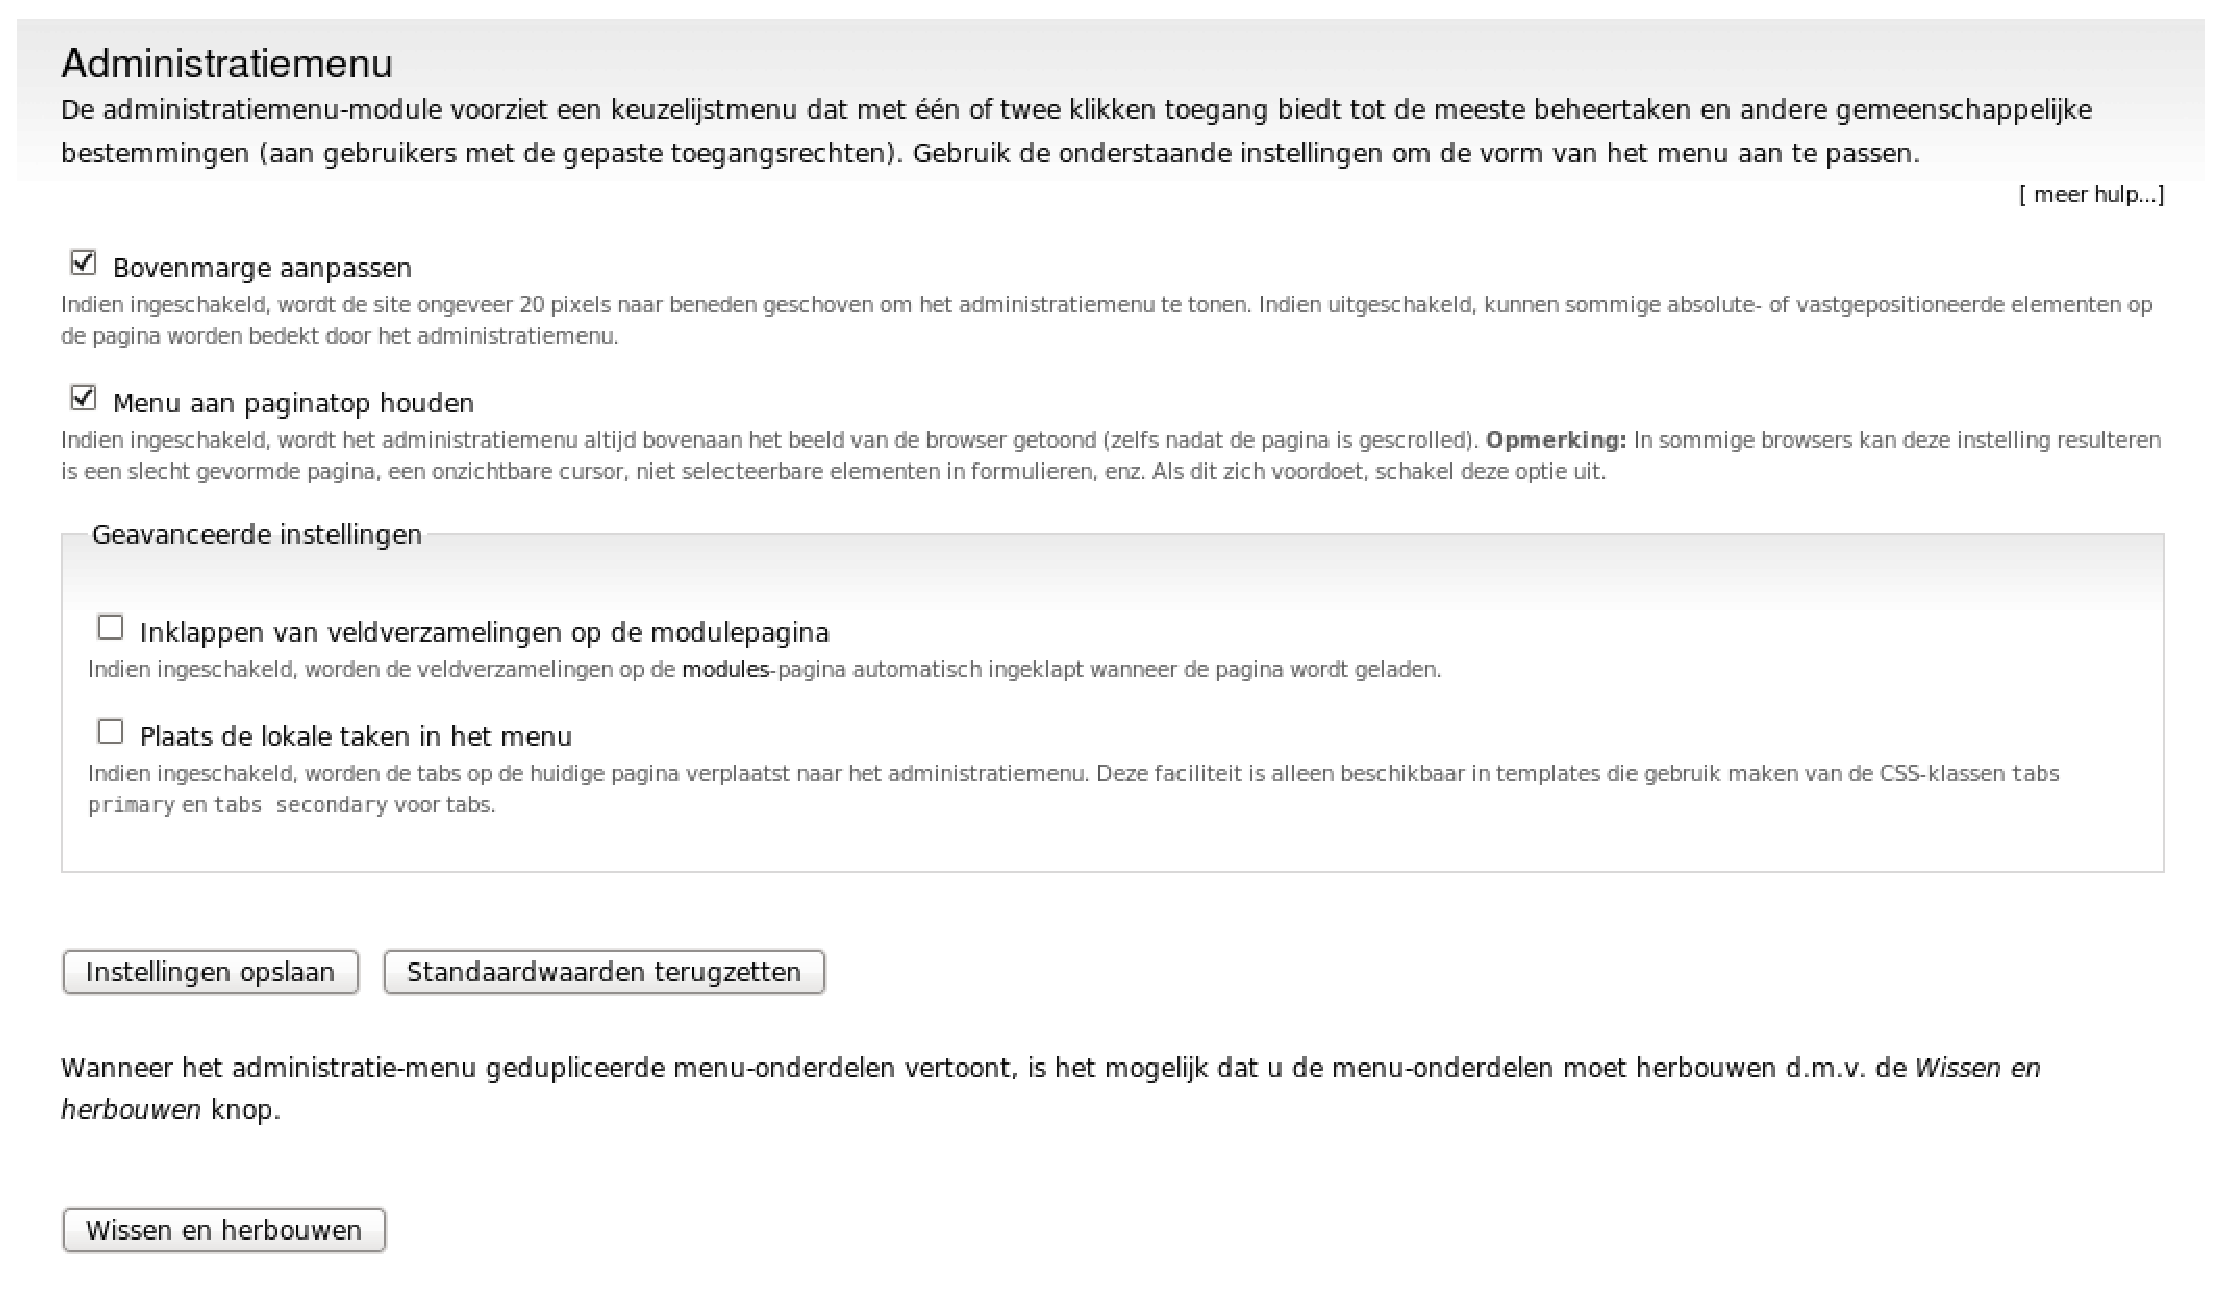
\includegraphics[scale=0.3,angle=0]{administratiemenu}
   \caption{administratiemenu.\label{white}}
 \end{figure}

\section{Beeldverwerkingstoolkit} \index{beeldverwerkingstoolkit}
Kies eventueel welke beeldverwerkingstoolkit gebruikt wordt als er meerdere
toolkits ge\"installeerd zijn. 
\begin{figure}[!h]
    \centering
   
\includegraphics[scale=0.3,angle=0]{beeldverwerkingstoolkit}
   \caption{beeldverwerkingstoolkit.\label{white}}
 \end{figure}
 
\section{Beheertemplate} \index{beheertemplate}
Hier kan men de lay-out van de beheerinterface instellen. Bepaal met
 welke template de beheerpagina's worden weergegeven. Als u de
 'Systeemstandaard' kiest, worden de beheerpagina's met de zelfde template als
 de rest van de site weergegeven.
\begin{figure}[!h]
    \centering
   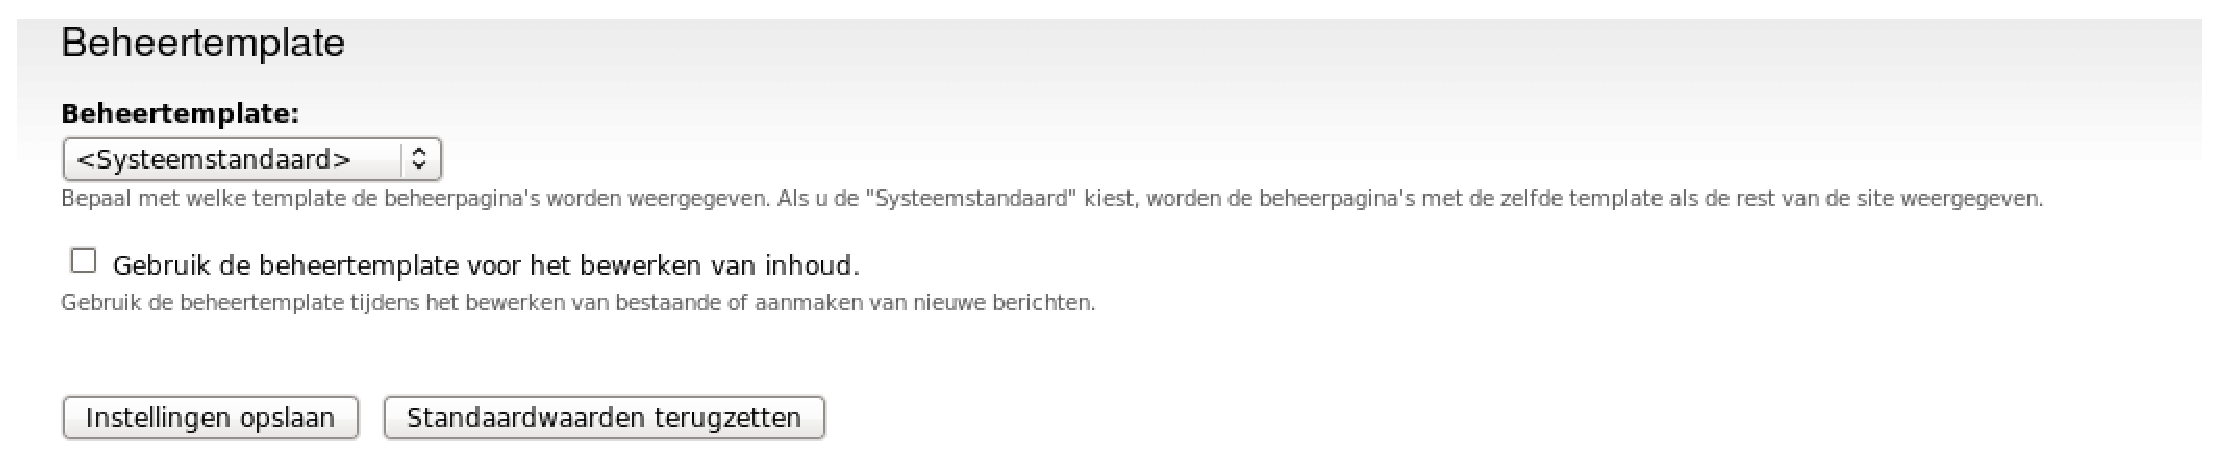
\includegraphics[scale=0.3,angle=0]{beheertemplate}
   \caption{beheertemplate.\label{white}}
 \end{figure} 
 
 
\section{Bestandssysteem} \index{bestandssysteem}
    Bepalen waar Drupal geuploade bestanden opslaat en hoe deze toegankelijk
    zijn. Een bestandssysteempad waar de bestanden zullen worden opgeslagen. De
    map moet bestaan en Drupal moet schrijftoegang hebben. Indien de downloadmethode publiek 
    is, dan moet deze map als relatief pad naar de Drupal-installatiemap worden opgegeven en 
    toegankelijk zijn via het internet. Indien de downloadmethode priv\'e is,
    dan mag de map niet te benaderen zijn via het internet. Indien u deze locatie wijzigt zullen alle downloadpaden wijzigen, 
    wat op een bestaande site onverwachte problemen kan opleveren.
 \begin{figure}[!h]
    \centering
   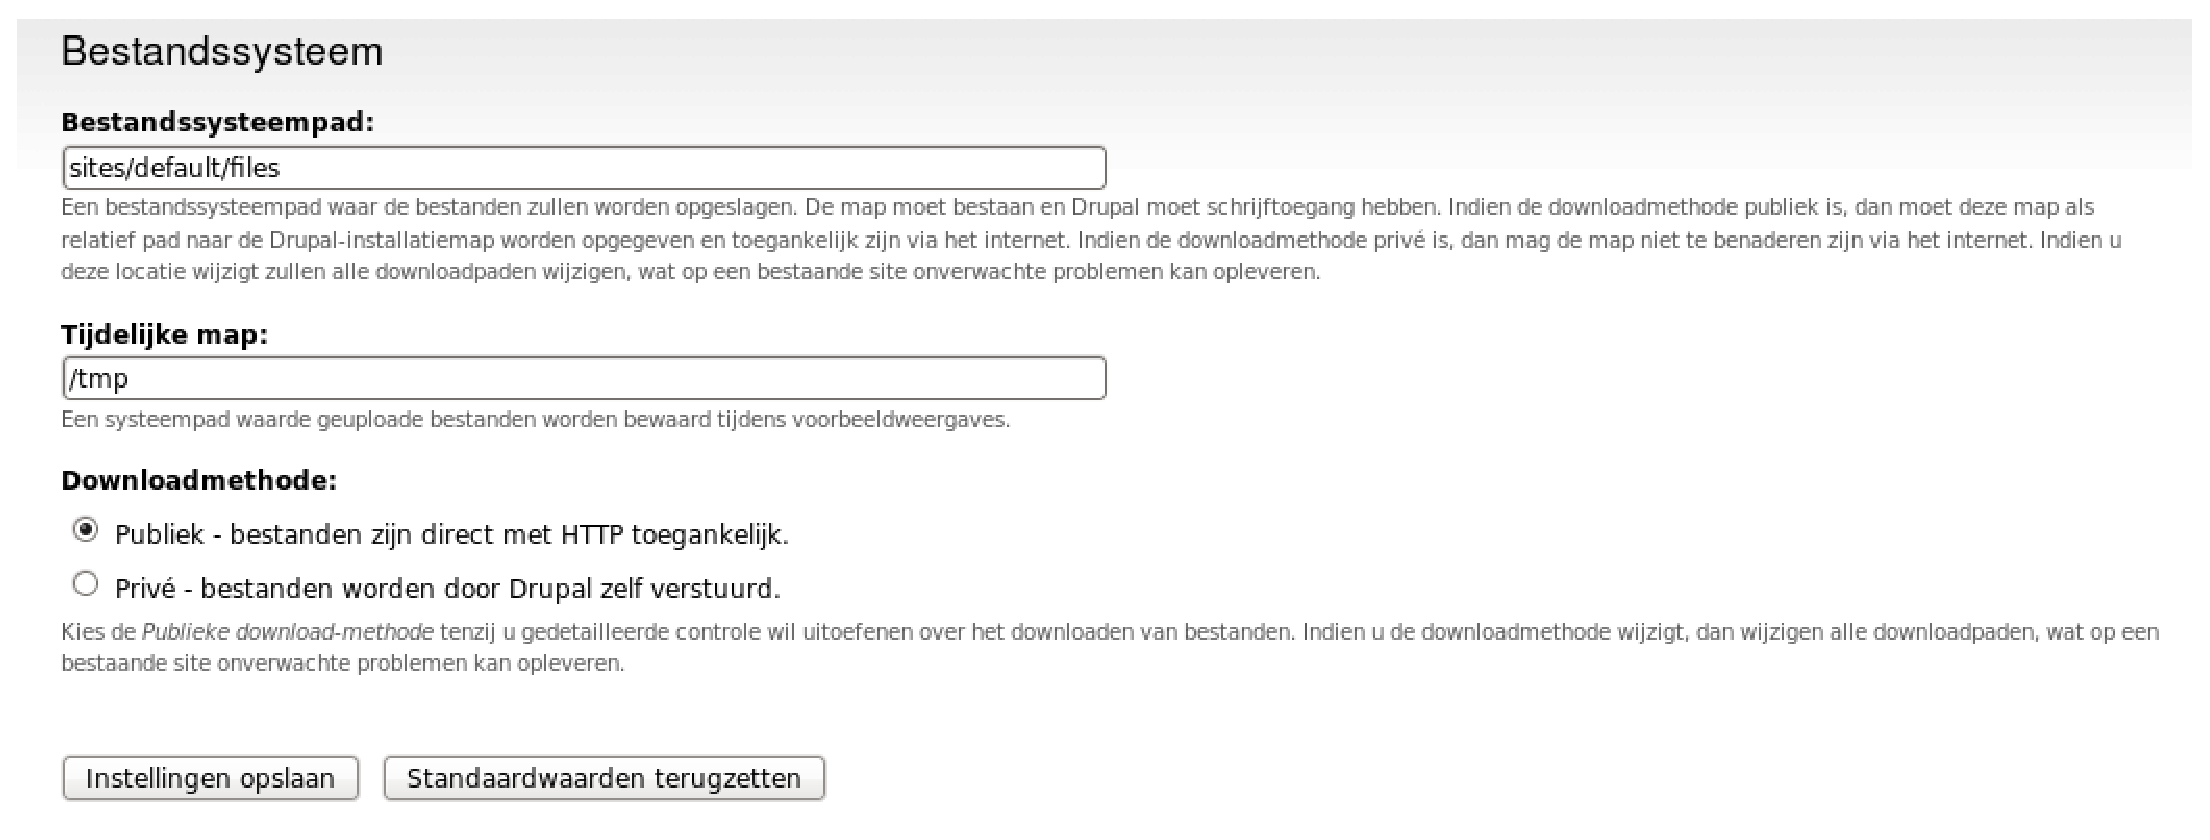
\includegraphics[scale=0.3,angle=0]{bestandssysteem}
   \caption{bestandssysteem.\label{white}}
 \end{figure}   
    
    
\section{Datum \index{datum} en tijd \index{tijd}} 
    Instellingen voor de weergave van datum en tijd en de standaard tijdzone van het Drupal systeem.
\begin{figure}[!h]
    \centering
   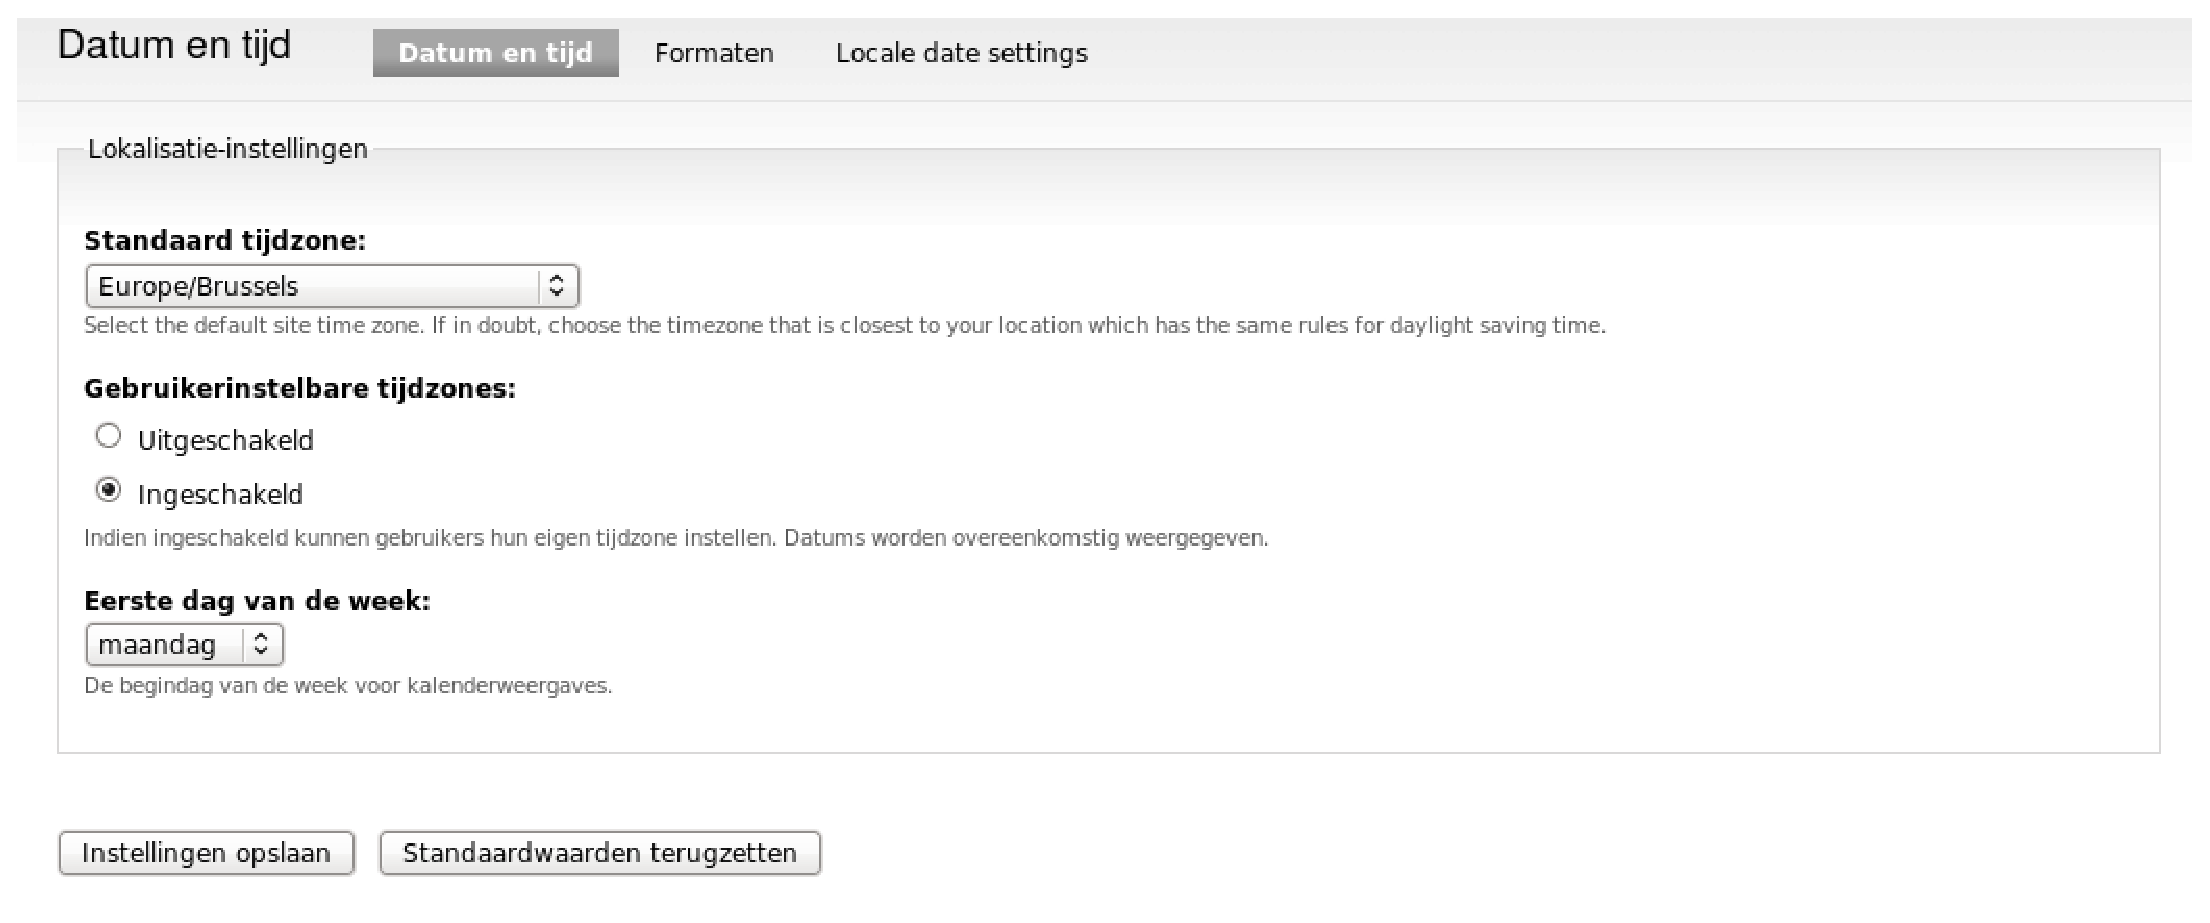
\includegraphics[scale=0.3,angle=0]{datum-tijd}
   \caption{datum-tijd.\label{white}}
 \end{figure}      
    
\section{Foutrapportage} \index{foutrapportage}
    Bepaal hoe Drupal omgaat met fouten, waaronder 403/404-fouten en PHP-foutrapportage.
 \begin{figure}[!h]
    \centering
   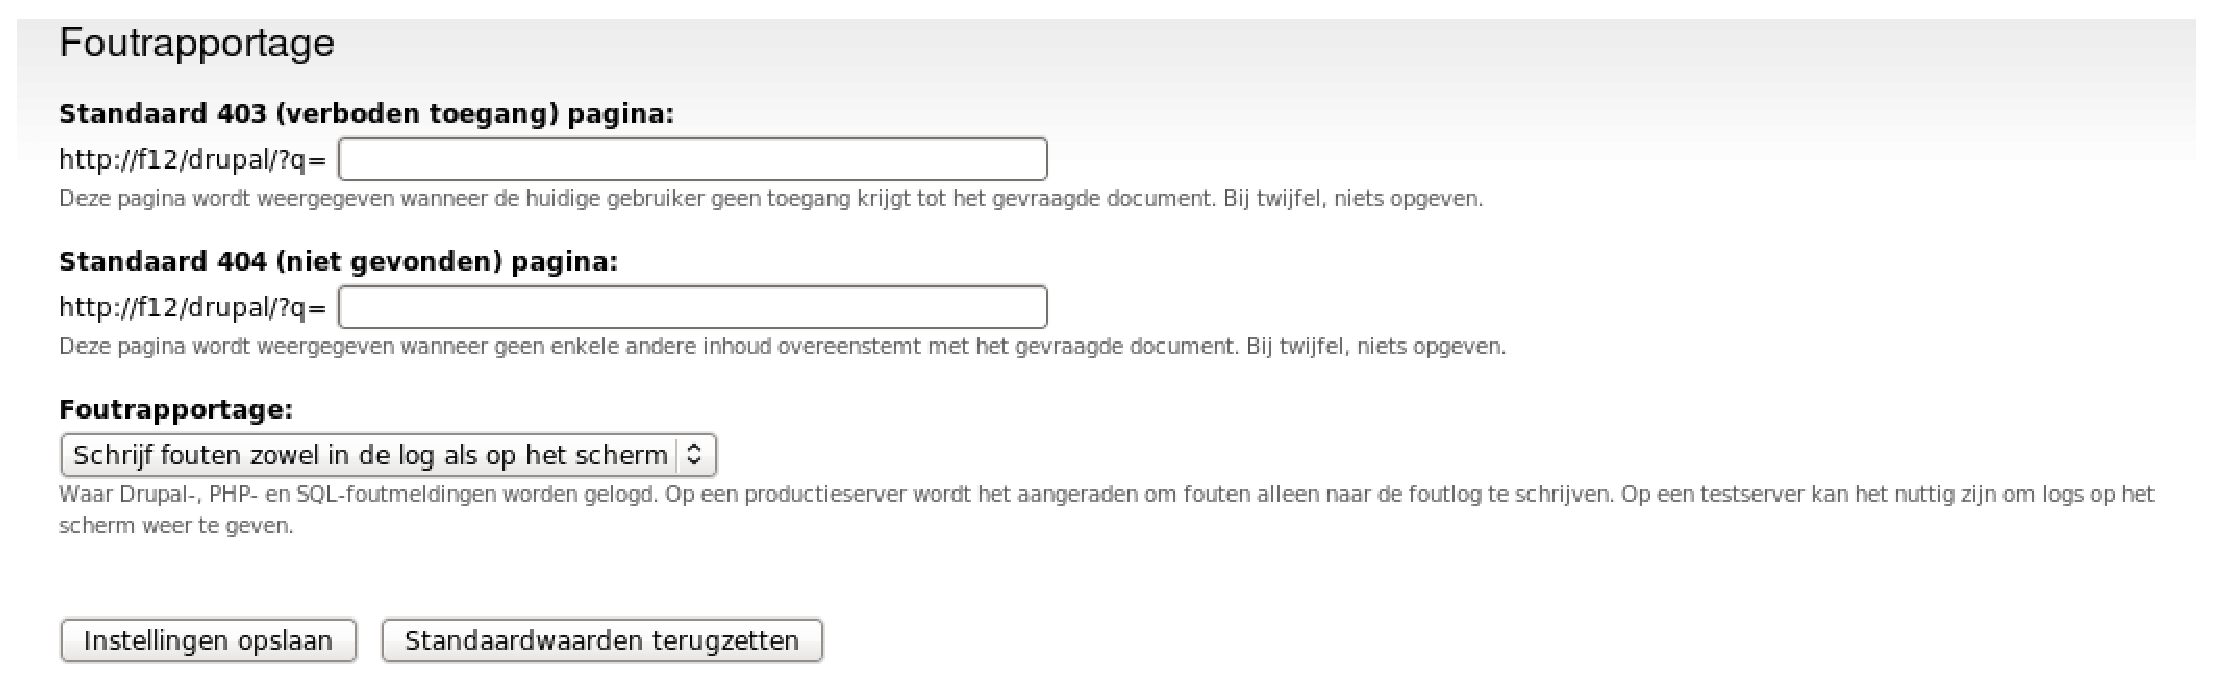
\includegraphics[scale=0.3,angle=0]{foutrapportage}
   \caption{foutrapportage.\label{white}}
 \end{figure}    
    
\section{Invoerformaten} \index{invoerformaten} 
    Bepaal hoe door gebruikers ingevoerde inhoud wordt gefilterd, inclusief toegestane HTML-tags. 
    Ondersteunt het inschakelen van filters die door modules worden aangeboden.
    \\
    Invoerformaten vormen het mechanisme waarmee Drupal de door gebruikers ingevoerde tekst verwerkt. 
    Ieder invoerformaat gebruikt filters om tekst te bewerken, de meeste invoerformaten passen meerdere 
    filters in een bepaalde volgorde toe. Ieder filter is voor een bepaald doel gebouwd en zal gewoonlijk 
    delen van de gebruikersinvoer verwijderen, omvormen of informatie toevoegen voordat deze wordt weergegeven. 
    Gebruikers kunnen tijdens het aanmaken of bewerken van inhoud tussen de beschikbare invoerformaten kiezen.
\\
Gebruik de onderstaande lijst om aan te geven welke invoerformaten voor welke rollen beschikbaar zijn en 
om het standaard invoerformaat te selecteren. Het standaardformaat is voor alle gebruikers beschikbaar. 
Voor gebruikers met toegangsrechten "filters beheren" zijn alle invoerformaten beschikbaar.
 \begin{figure}[!h]
    \centering
   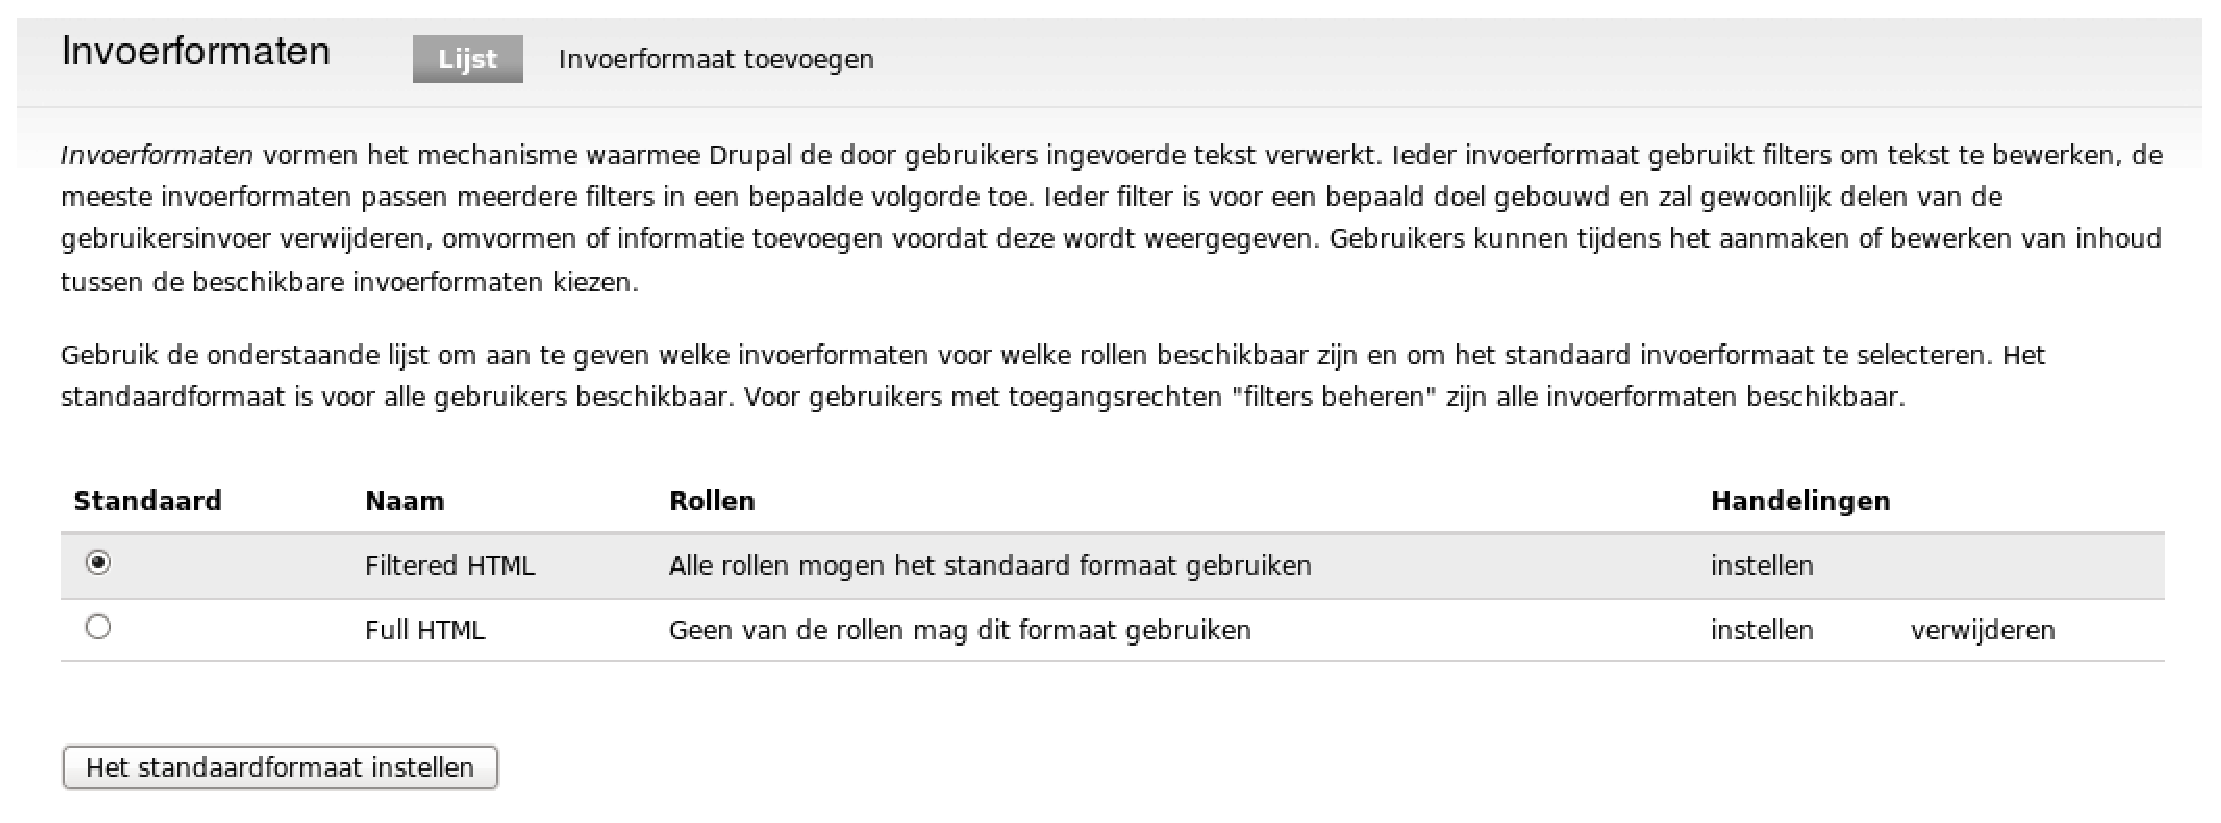
\includegraphics[scale=0.3,angle=0]{invoerformaten}
   \caption{invoerformaten.\label{white}}
 \end{figure}     
    
    
\section{Loggen \index{loggen} en waarschuwingen \index{waarschuwingen}} 
    Instellingen voor het logboek \index{logboek} en alarmmodules
    \index{alarmmodules}. Verschillende modules kunnen Drupals
    systeemgebeurtenissen doorsturen naar verschillende bestemmingen (het systeemlogboek, een database, e-mail, enz.). Dit is de meest gebruikelijke methode for kleine
    tot middelgrote sites op shared hosting. De logs kunnen op de beheerpagina's worden bekeken.
\begin{figure}[!h]
    \centering
   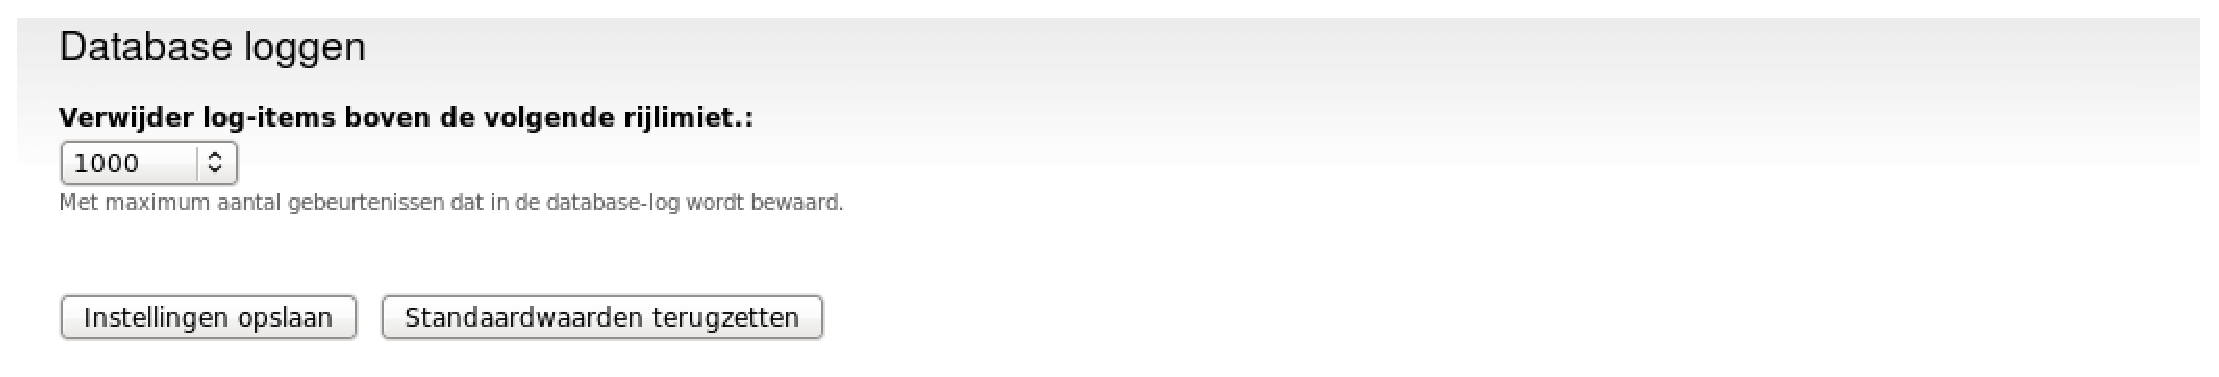
\includegraphics[scale=0.3,angle=0]{database-loggen}
   \caption{database-loggen.\label{white}}
 \end{figure}       
    
    
\section{Prestatie} \index{prestaties}
    Pagina-cache voor anonieme gebruikers in of uitschakelen en CSS- en JS-bandbreedte-optimalisatie instellingen.
\subsection{Pagina-cache} \index{pagina-cache} 
De pagina-cache inschakelen leidt tot significant betere prestaties. Drupal kan
  gecomprimeerde cache-pagina's bewaren en deze tonen aan anonieme gebruikers. Door een pagina op te slaan in de 
  cache hoeft Drupal deze pagina niet bij elk bezoek opnieuw op te bouwen.
\begin{figure}[!h]
    \centering
   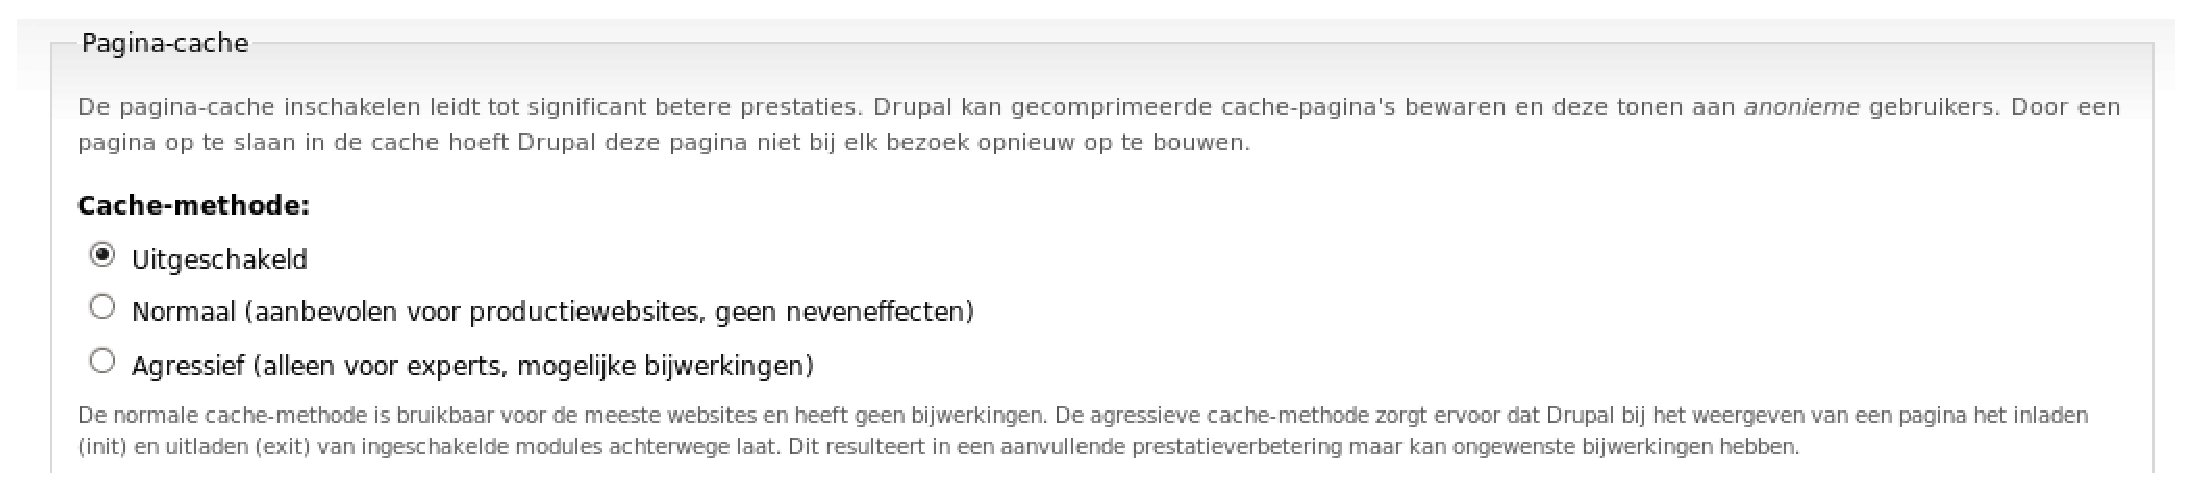
\includegraphics[scale=0.3,angle=0]{prestatie-pagina}
   \caption{prestatie-pagina.\label{white}}
 \end{figure} 
\subsection{Blok-cache} \index{blok-cache}
  Door de blok-cache in te schakelen kunnen gebruikers een prestatieverbetering
  merken; u voorkomt zo dat blokken bij elke raadpleging van een pagina opnieuw opgebouwd worden. 
  Indien de pagina-cache ook is ingeschakeld dan zal de blok-cache vooral geregistreerde gebruikers ten goede komen.
\begin{figure}[!h]
    \centering
   
\includegraphics[scale=0.3,angle=0]{prestatie-blok}
   \caption{prestatie-blok.\label{white}}
 \end{figure}
\subsection{Bandbreedte-optimalisaties} \index{bandbreedte}
\index{optimalisaties} Drupal kan automatisch externe bronnen zoals CSS en JavaScript optimaliseren,
wat zowel de grootte als het aantal aanvragen aan uw website kan verminderen. CSS-bestanden kunnen samengevoegd 
en gecomprimeerd worden tot \'e\'en enkel bestand, terwijl JavaScript-bestanden
samengevoegd (maar niet gecomprimeerd) worden. Deze optimalisaties zijn optioneel en kunnen de serverbelasting, benodigde bandbreedte en paginalaadtijden verminderen.
\begin{figure}[!h]
    \centering
   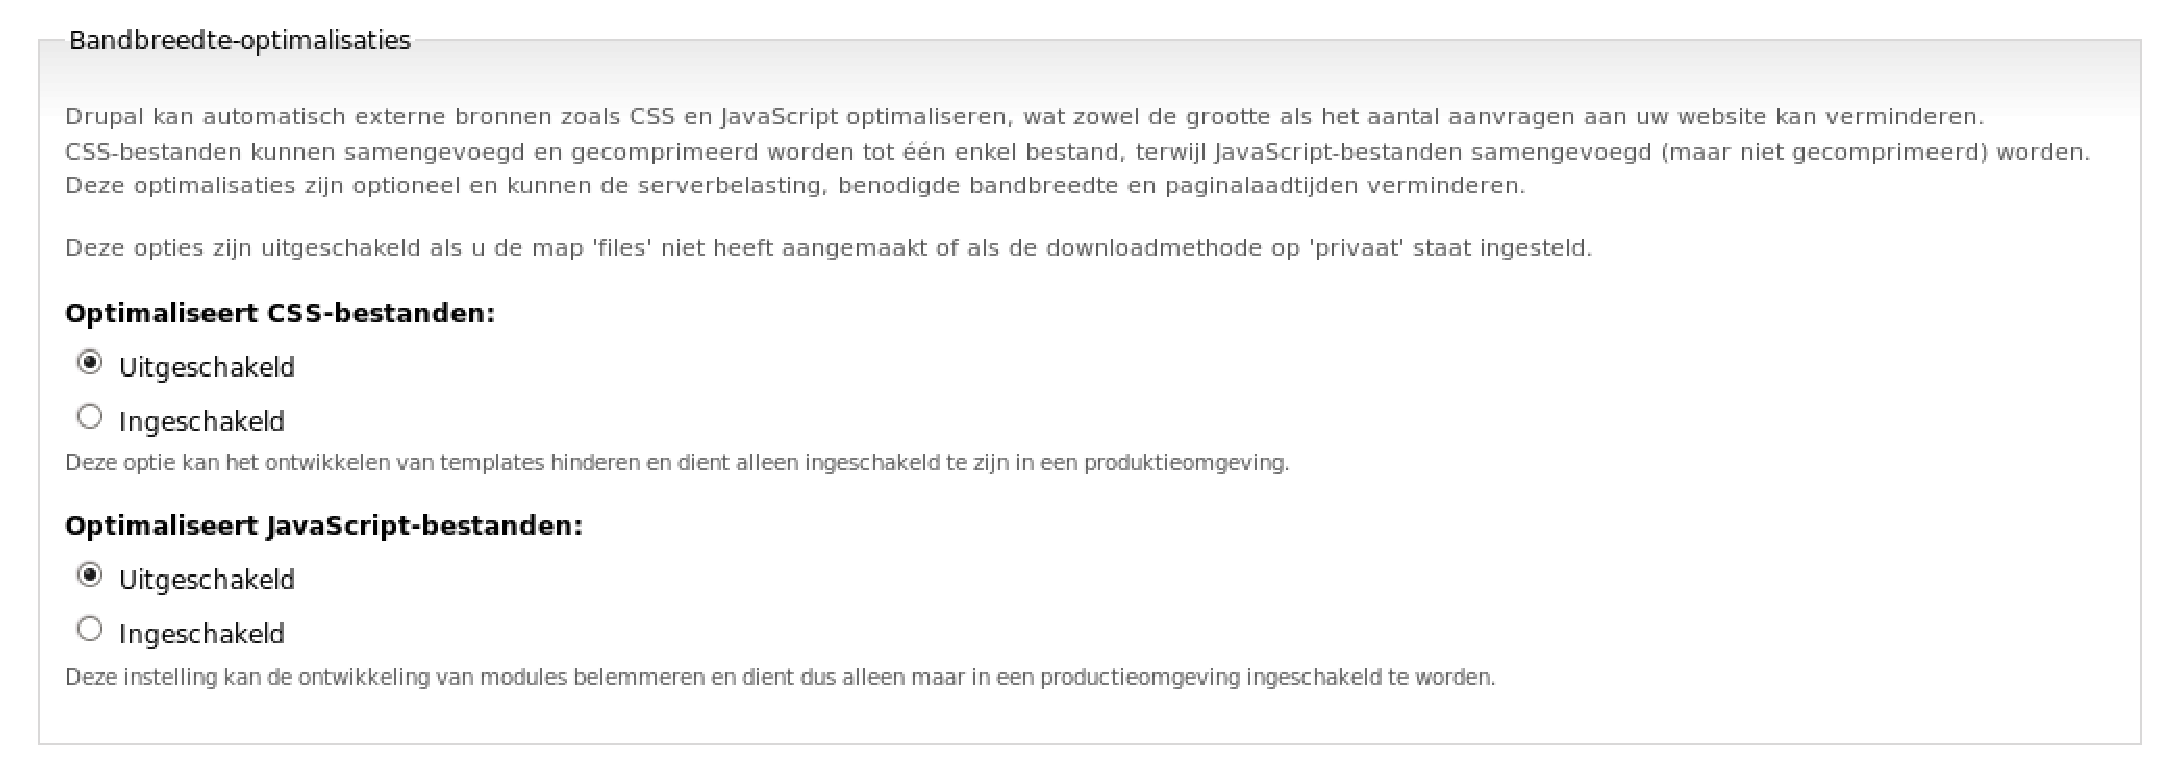
\includegraphics[scale=0.3,angle=0]{prestatie-bandbreedte}
   \caption{prestatie-bandbreedte.\label{white}}
 \end{figure}
\subsection{Cache-data opschonen} \index{cache-data}
Bufferen van gegevens verbetert de prestaties van de website, maar kan problemen
opleveren tijdens foutzoeken in nieuwe modules, templates of vertalingen als verouderde informatie wordt gebufferd. 
Klik op de onderstaande knop om alle gebufferde informatie op de site te verversen. Websites met veel dataverkeer zullen 
merkbaar langzamer reageren gedurende het opbouwen van de cache.
\begin{figure}[!h]
    \centering
   
\includegraphics[scale=0.3,angle=0]{prestatie-cache}
   \caption{prestatie-cache.\label{white}}
 \end{figure}
 
\section{Schone URL's} \index{url}
    Schone URL's in- of uitschakelen. Deze optie zorgt ervoor dat Drupal
    'schone' URL's gebruikt (d.w.z. zonder ?q= in de URL.) 
\begin{figure}[!h]
    \centering
   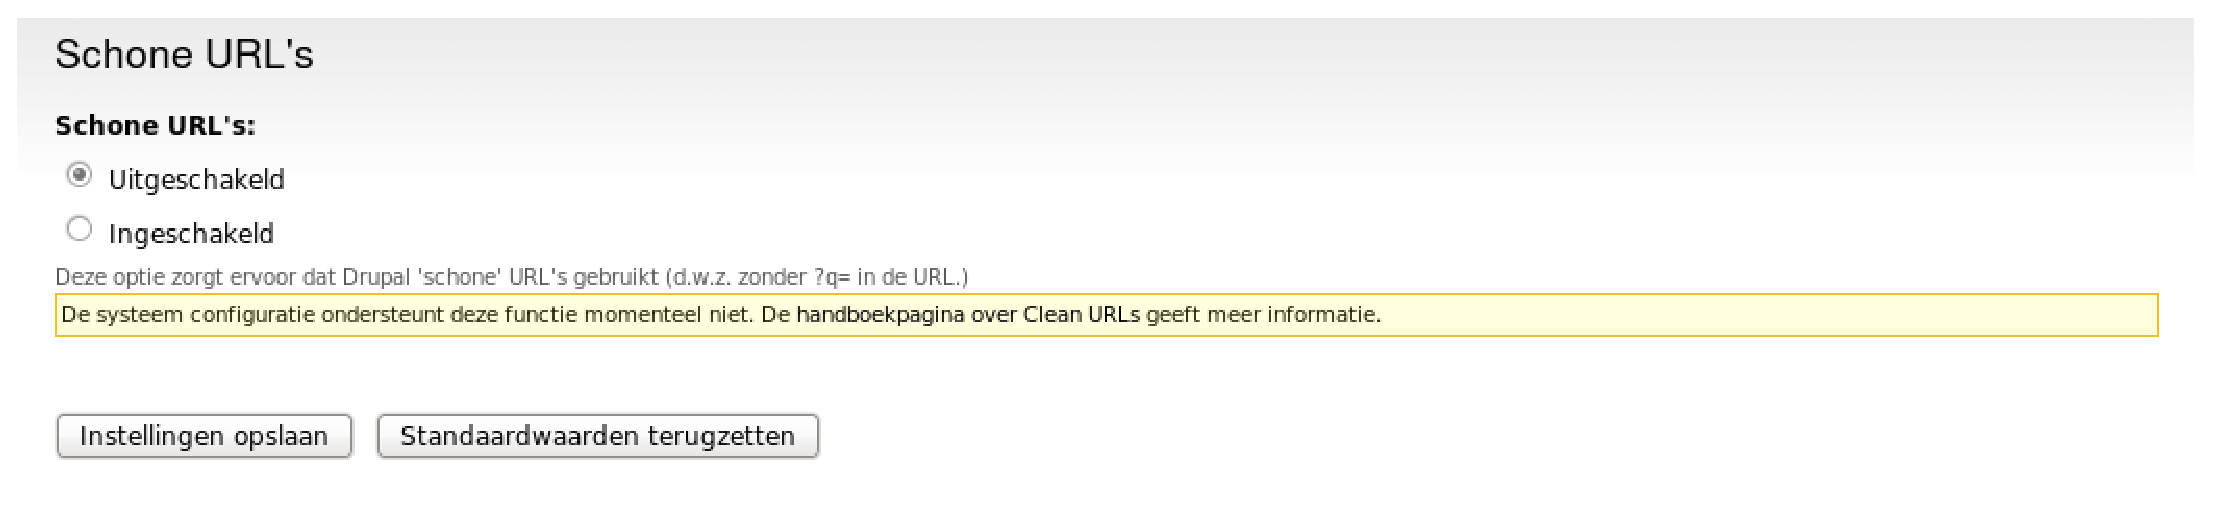
\includegraphics[scale=0.3,angle=0]{schone-urls}
   \caption{schone-urls.\label{white}}
 \end{figure}

\section{Site-onderhoud} \index{onderhoud}
    Website offline brengen voor onderhoud of opnieuw online brengen. Als
    'Online' \index{online} is ingesteld, kunnen alle bezoekers uw site gewoon
    bezoeken. Als 'Offline' \index{offline} is ingesteld, kunnen alleen
    gebruikers met de 'Site-instellingen beheren' rechten uw site bezoeken om onderhoud te verrichten. Alle andere
    bezoekers zullen het off-line bericht zien dat u hieronder kunt instellen. 
    Geauthoriseerde gebruikers kunnen tijdens de 'Off-line' modus inloggen via
    de inlogpagina.
 \begin{figure}[!h]
    \centering
   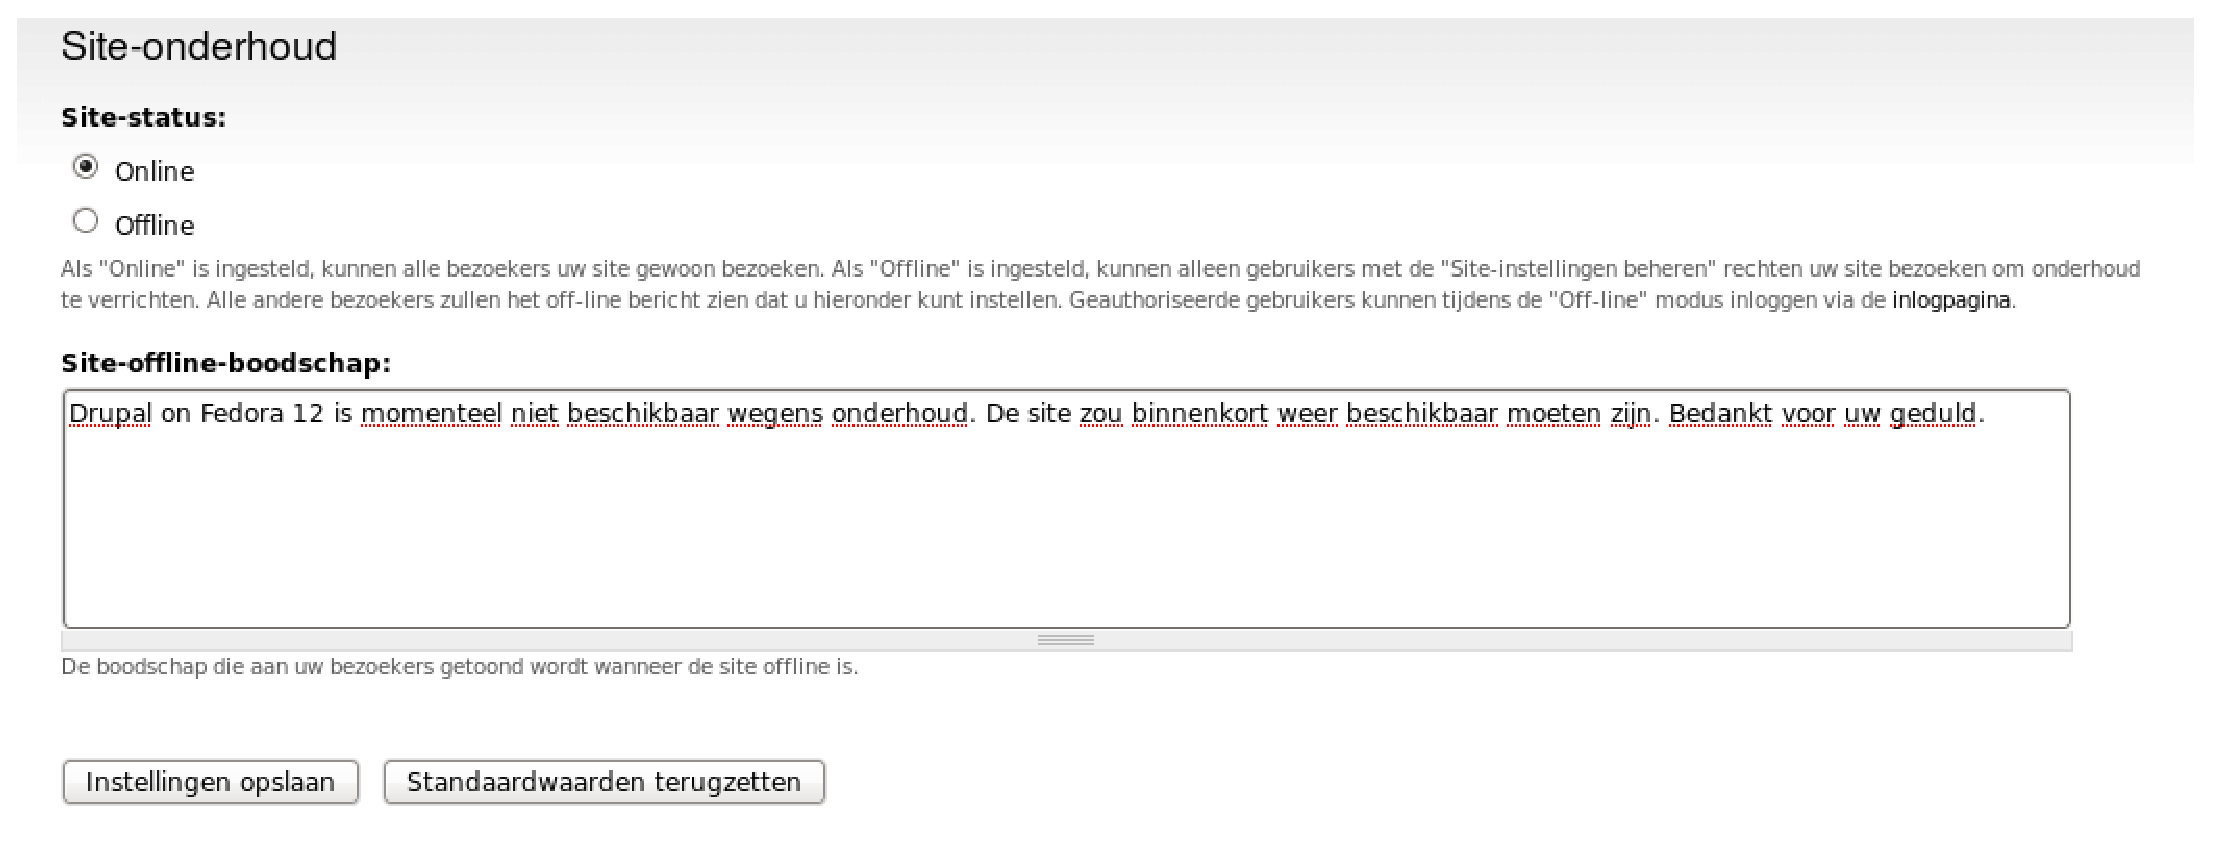
\includegraphics[scale=0.3,angle=0]{site-onderhoud}
   \caption{site-onderhoud.\label{white}}
 \end{figure}   
    
\section{Talen} \index{talen}
    Instellingen voor de taal van inhoud en gebruikersinterface. \\
Wanneer meerdere talen zijn 
ingeschakeld, kan de tekst van de website-interface worden vertaald, kunnen geregistreerde 
gebruikers op de pagina Mijn account de taal van hun keuze instellen en kunnen auteurs de 
taal aangeven waarin de pagina-inhoud wordt ingediend. De standaardtaal wordt gebruikt voor 
anonieme gebruikers en voor gebruikers die geen voorkeurstaal hebben opgegeven.
\\
Voor iedere op de site beschikbare taal gebruikt u de link bewerken om de taal te configureren; 
waaronder naam van de taal, taalspecifiek pad of domein en de schrijfrichting van de 
taal (Links-naar-Rechts of Rechts-naar-Links). Deze talen zijn ook beschikbaar in de 
Taalkeuze bij het aanmaken van pagina's van inhoudstypen die meertaligheid ondersteunen.
\\
Gebruik de pagina Taal toevoegen om extra talen in te schakelen (en indien beschikbaar 
het vertaalpakket automatisch te importeren).\\ De pagina Vertalen om lokale
tekenreeksen te vertalen of de pagina Importeren om vertalingen uit losse .po-bestanden toe te voegen. 
Vertaalpakketten vindt u op de Drupal.org Translations-pagina.
\index{translation} \begin{figure}[!h]
    \centering
   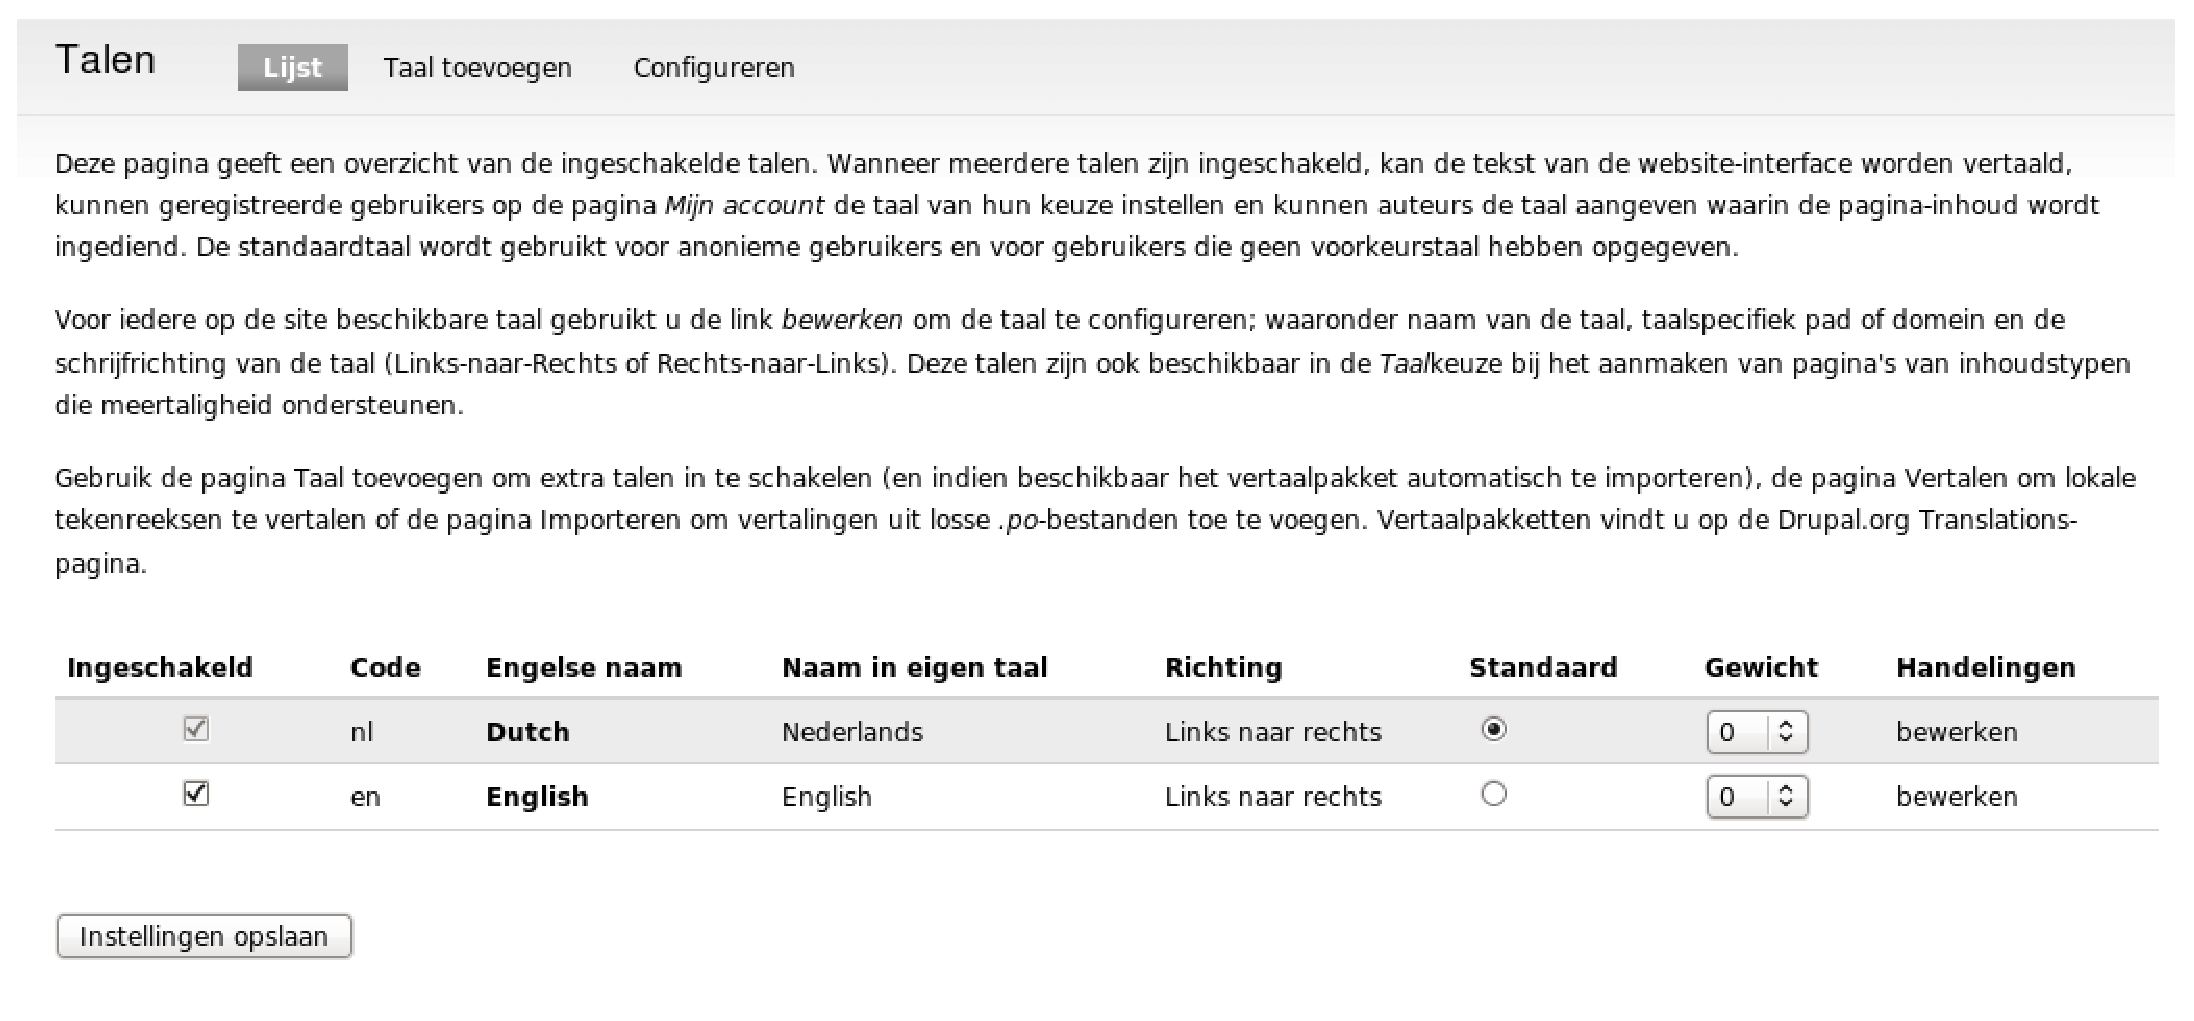
\includegraphics[scale=0.3,angle=0]{talen}
   \caption{talen.\label{white}}
 \end{figure} 

\section{ Websitegegevens} \index{websitegegevens}
    Basis website gegevens instellen zoals naam van de site \index{naam},
    slogan \index{slogan}, e-mailadres, voorpagina \index{voorpagine}, enz.
    \begin{figure}[!h]
    \centering
   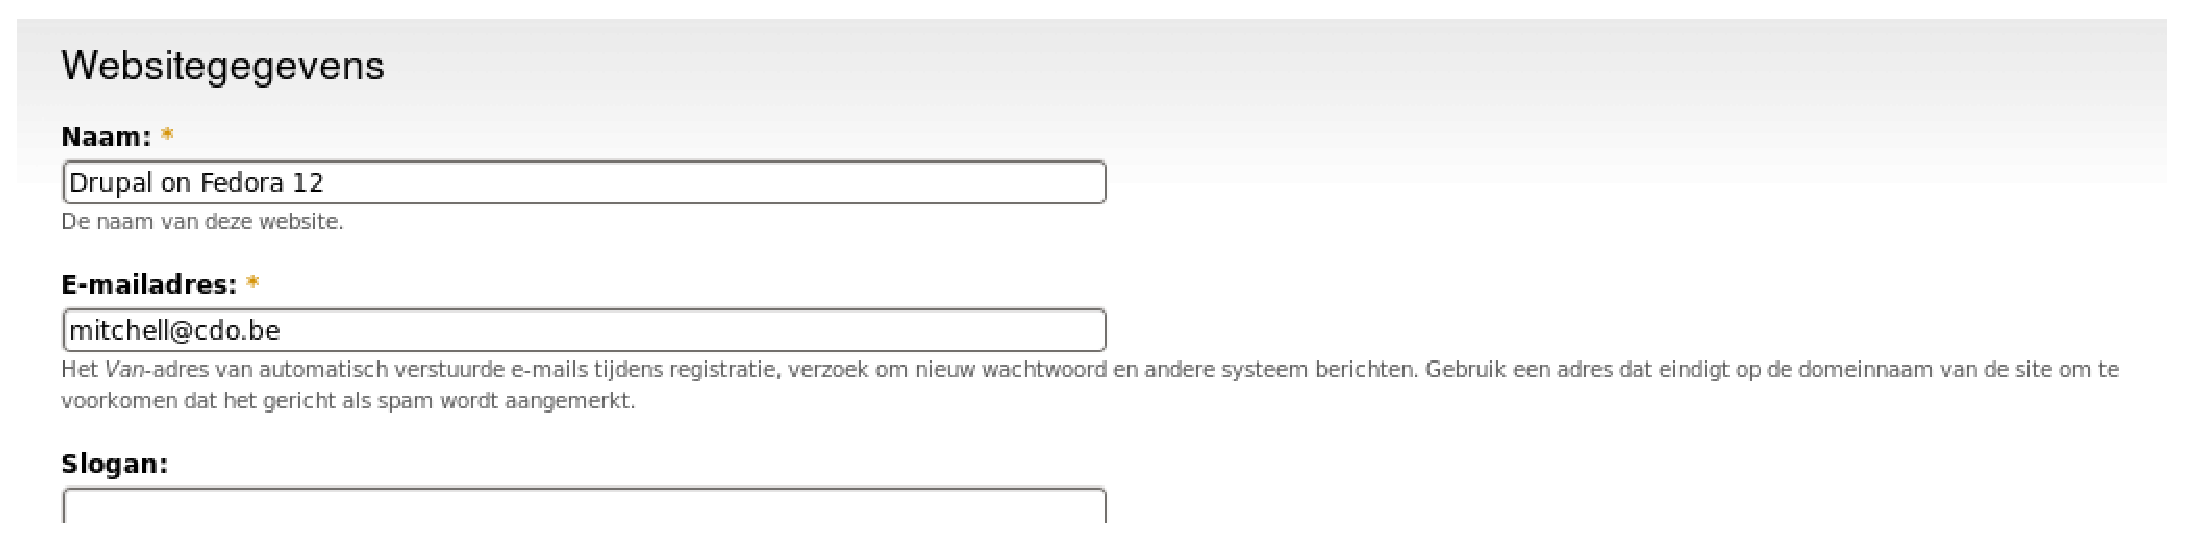
\includegraphics[scale=0.3,angle=0]{website-gegevens}
   \caption{website-gegevens.\label{white}}
 \end{figure}    
    
\section{Zoekinstellingen} \index{zoekinstellingen}
    Relevantie voor zoeken en andere indexeerinstellingen
    \index{indexeerinstellingen}. De Search-module \index{search-module} biedt
    de mogelijkheid om de inhoud van de site op trefwoord te doorzoeken. Zoeken is vaak de enige praktische manier om informatie op een grote site te vinden en kan voor het vinden van gebruikers en inhoud van de site worden toegepast.
\\
Om het zoeken op de website mogelijk te maken houdt de Drupal-zoekmachine een index bij 
van woorden die voorkomen in de inhoud van de site. Voor het opbouwen en bijhouden 
van deze index is cron nodig. Het indexeergedrag kan worden ingesteld op de pagina 
Zoekinstellingen. Op deze pagina kan het Aantal items dat per cron-uitvoering
wordt ge\"indexeerd worden ingesteld. Verminder dit aantal om timeout- en
geheugenfouten tijdens het indexeren te voorkomen.
  \begin{figure}[!h]
    \centering
   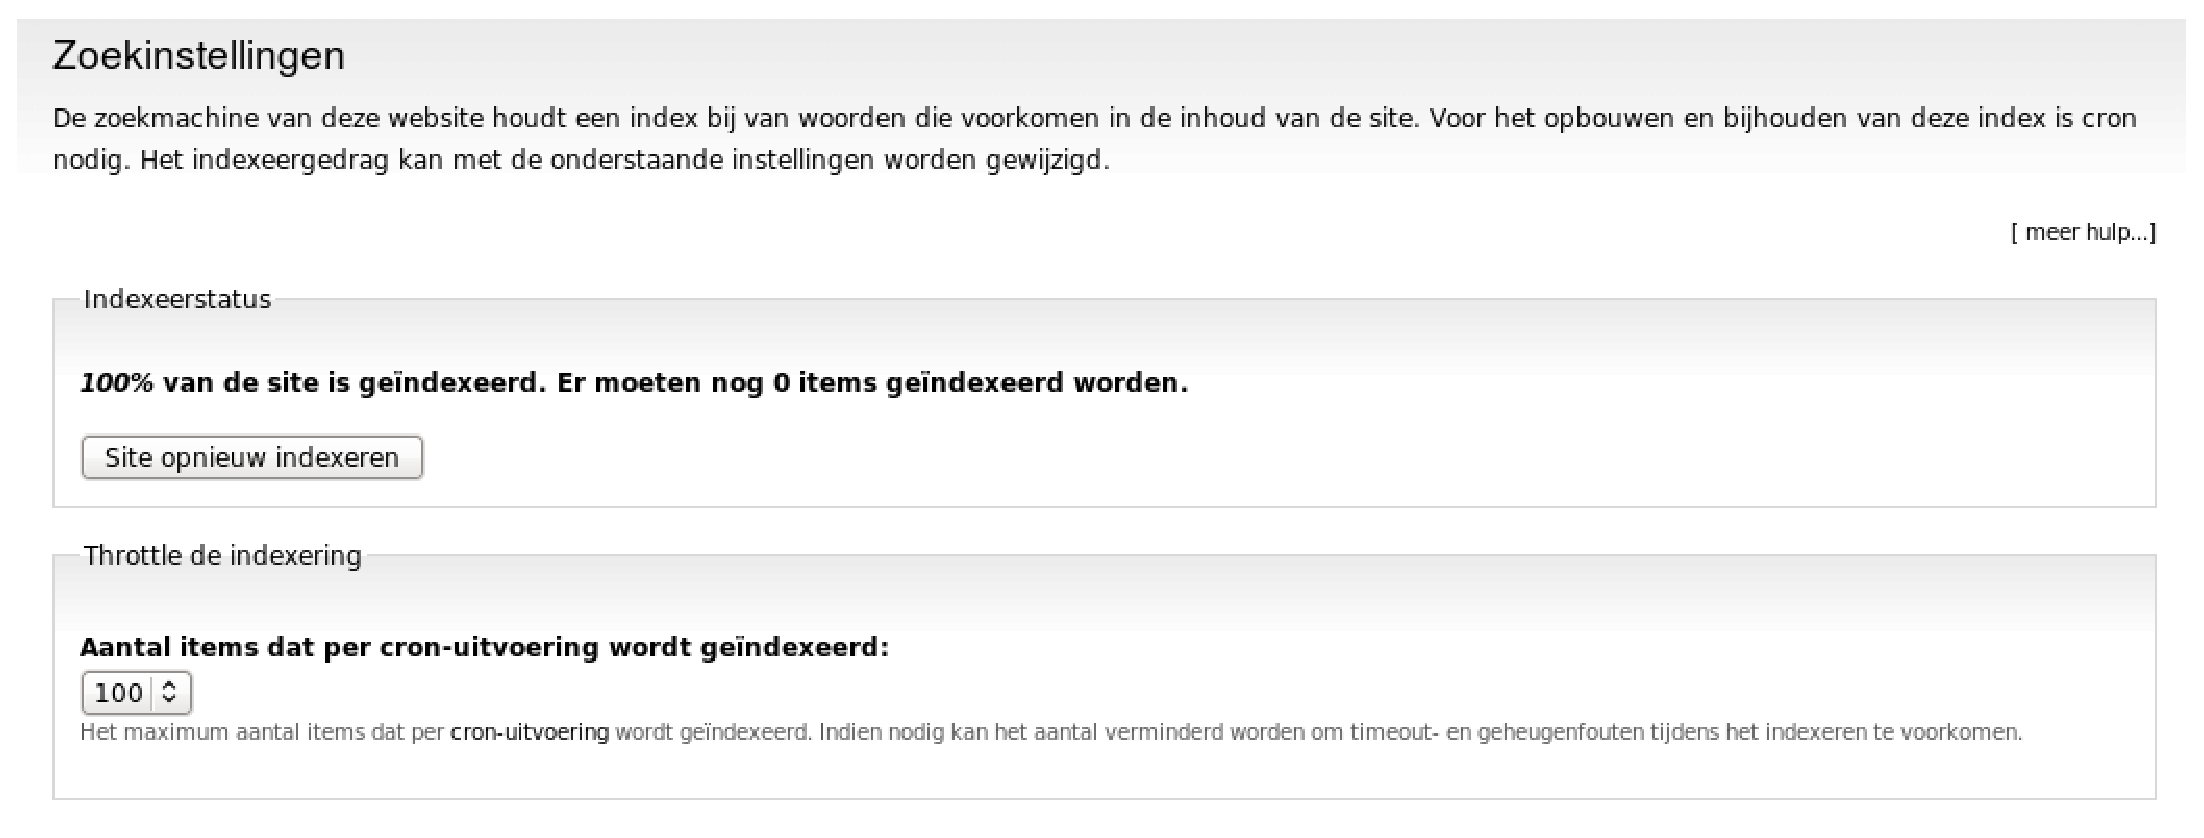
\includegraphics[scale=0.3,angle=0]{zoekinstellingen}
   \caption{zoekinstellingen.\label{white}}
 \end{figure}